
% LaTeX template document 
% Samuel Regandell 2003,2004
% Lines after '%' are commented out. '\' begins a command. 
% [...] indicate optional parameters. {...} indicate mandatory parameters.


% ============================================================================================= Preamble

%----------------------------------------- class of document
% documentclass[option,option, ...]{class}
% classes: article (for scientific reports/docs/invitations etc OBS-no chapters!)
%          report  (longer reports w.everal chapters/small books/PhD theses)
%          book    (real books)
%          slides  (for slides-with big letters/better use FoilTeX)

% options: 10pt,11pt,12pt                  (size of main font - default is 10pt)
%          draft                           (marks ``ugly'' typesetting results with black lines)
%          a4paper,letterpaper,a5paper etc (papersize - default is letterpaper)
%          fleqn                           (formulae is left-alligned, not centered)
%          leqno                           (formulae numbers on left, not right)
%          titlepage,notitlepage           (title on separate page or not)
%          onecolumn,twocolumn             (one- or two-column document)
%          landscape                       (changes page orientation)
%          openright,openany               (if next chapter will begin only on right-hand sides or not -
%  				            defaults differently in book and report; not available in article)							   
\documentclass[a4paper,12pt,notitlepage,twocolumn]{article}

% ---------------------------------------- page & text settings

% pagestyle{style}     (hint: to change style in current page, use \thispagestyle{style} )
% styles:   plain      (page-nr in footer; default setting)   
%           headings   (chapter & page-nr in header, no footer)
%           empty      (header & footer empty)

 \pagestyle{empty}

% linespread{factor} 
% factors:  1          (default line spacing)
%           1.3        (1.5 line spacing)
%           1.6        (double line spacing)

% \linespread{1.3}

%----------------------------------------- packages to load

% (See http://www-sop.inria.fr/miaou/latex/styles-eng.html for other packages.)

% usepackage[options,options, ...]{package} (packages for inserting graphics,language support etc)   


% \usepackage[swedish]{babel} % (swedish language support)
% \usepackage[T1]{fontenc}    % (swedish letters)

 \usepackage{graphicx}       % (allows postscript pictures in text with \includegraphics{file})   
% \usepackage{amssymb}        % (adds particular binary math symbols
                              %  such as ``approx.equal to'' etc.)
 \usepackage{fullpage}       % (reduces horisontal margins)
% \usepackage{makedx}         % (indexing system, activate with *Preamble* command \makeindex)

% \usepackage[options]{hyperref} % (should be *last* among packages to load)
                                 % (Allows for the creation of hyperlinks
                                 %  for use with e.g. latex2html or ps2pdf.
                                 %  In text, use \href{URL}{Name} or \url{URL}.        				 
                                 %  http://www.tug.org/applications/hyperref/manual.html)

%----------------------------------------- files to include

% \includeonly{filename,filename,...}   % (limits the files to be inserted later-better typesetting)

% ---------------------------------------- hyphenation rules 

% hyphenation(Hy-phen-a-thion Samuel) % (defines how to hyphenate ``hyphenation'', while  
                                      %  *never* hyphenating ``samuel'' or ``Samuel'').                                % \hyphenation{word list}

% ---------------------------------------- self-defined macros/definitions

% \newcommand{\new_command_name}[nr_of_args]{command_sequence or text}    % (nr_of_args defaults to 0)
% \newenvironment{\new_env_name}[nr_of_args]{process_run_before_environment}{process_run_after_environment}


%\renewcommand{\caption}[1]{\caption{\tiny $1}}

% ---------------------------------------- title page setup

\title{TriPlanetary Advanced}
\author{Griatch (www.griatch-art.deviantart.com)}   % (separate several authors with \and)
%\date{}   % (for no date, put date field blank)


% ============================================================================================= Document Begin
\begin{document}


% ---------------------------------------- create title,TOC etc 

%\maketitle                   % (document title - specified above - is placed here)
%\tableofcontents            % (document might have to be run two-three times to get TOC right.)
                             % (add '*' after section command to have it not appear in TOC)
%\listoffigures
%\listoftables

% --------------------------------------- main text -------------------------------------------

\section*{\center TriPlanetary Advanced\\by Griatch \\
   {\small (www.griatch-art.deviantart.com)}\\ {\small v0.5, April 2010}}

\section{Introduction}
Triplanetary Advanced (henceforth \emph{TriAv}) is a
space-combat game for two or more players. It simulates the physics of
space travel in two dimensions along the ecliptica of our solar
system. 
\\\\
TriAv expands on the since long out-of-print boardgame \emph{Triplanetary}
by GDW\footnote{Triplanetary's
  copyright currently belongs to Steve Jackson Games. Triplanetary
  Advanced is purely a unofficial fan expansion.}.
 TriAv takes the excellent movement rules from the original and
expands it quite considerably when it comes to weapons, hit damage and ship
design. This document completely replaces the old Triplanetary manual.

\section{Game components}
TriAv comes as three separate files which you are encouraged to
print copies of. TriAv also requires a normal 6-sided die (often
called a \emph{d6}). 
\label{sec:game_components}
\begin{itemize}
\item The \emph{TruAv manual} is what you are currently reading. It
  contains all the rule details but you will likely not have to refer
  much to it once you've played a game or two. 
\item \emph{The solar system map} acts as the playing
  field for the game. TriAv is played by drawing ship 
  vectors on this hexagonal gridded map using normal pencils. Whereas
  you can laminate a copy of this map and use erasable grease pencils,
  we find it's easiest to just print out a few paper copies and draw
  directly on them. The map can easily, and usually cheaply, be printed
  to A3 size (or bigger with a commercial printer).
\item  \emph{The game-aid} folds into three parts and contains the ship
  manifest and all tables needed for play. Each player gets one of
  these for each ship they control.  
\end{itemize} 
TriAv does not use any counters. We find this makes it very portable and
easy to play on the move. It is also easy to pause and continue at a
later time. If you have problems with the map getting messy (this can
happen when there are many ships), consider using coloured pencils to
separate tracks. Other 
inventive suggestions are to experiment with counters like in the
original Triplanetary or by placing the map on a whiteboard and use
small magnets to mark ships.   

\section{Sequence of play}
\label{sec:sequence_of_play}
Each player performs all the following steps in order before it's the
next player's turn. Player order can be jointly agreed upon or decided
randomly. In game terms, each turn is assumed to last about
a day. Of these phases, only Astrogation and Movement are mandatory. 
\begin{enumerate}
\item \emph{Astrogation phase}: The player plots the future location
  of their ships, taking into account the effect of
  gravity and if they want to burn fuel to change their vector. Also
  the vectors of previously launched weapons are plotted. Note that no
  object is actually yet moved in this phase.  
\item \emph{Launch phase}: Weapons that require time to reach their
  target (such as mines and all types of missiles) are launched and
  their vectors plotted (but not actually moved yet). They
  inherit the old vector of their launching ship plus eventual adjustments
  they are themselves capable of.  
\item \emph{Movement phase}: The ship and launched weapons now move along
  their plotted vectors to their new positions. If launched weapons hit
  something, damage is decided by die roll.
\item \emph{Gun fire phase}: The ship's mounted weapons (guns, lasers)
  fire against a target, taking into respect distance and
  relative velocities. Hits are decided by die roll. Targeted ships with guns 
  of their own may retaliate directly if they are capable. 
\item \emph{Resupply phase}: Ships capable to do so may refuel,
  load/unload cargo and other actions which might be determined by the
  scenario.
\end{enumerate}

\section{Astrogation}

\subsection{Basic movement}

\label{sec:astrogation}
TriAv simulates Newtonian movement in two dimensions. Each ship
has an intrinsic velocity represented by a straight-line arrow (this
is called a vector). The arrow has its tail at the location of the
ship at the beginning of the turn and points to the location it will
be at the end of the turn. A vector is always drawn between the
\emph{centers} of hexes. The basic rule of movement is: 
\begin{quotation}\noindent \emph{Any ship or other object not
        accelerated by thrust or gravity will move as it did on the
        previous turn and in the same direction.\footnote{In another
          form this is also known as Newton's first law.}}
\end{quotation}

By burning a point of fuel, a ship can shift the endpoint of its
vector by one hex in any direction. A ship may only burn one unit of
fuel per turn. A ship with zero speed is marked with a simple dot on the map.

\begin{figure}[h!]\centering  
  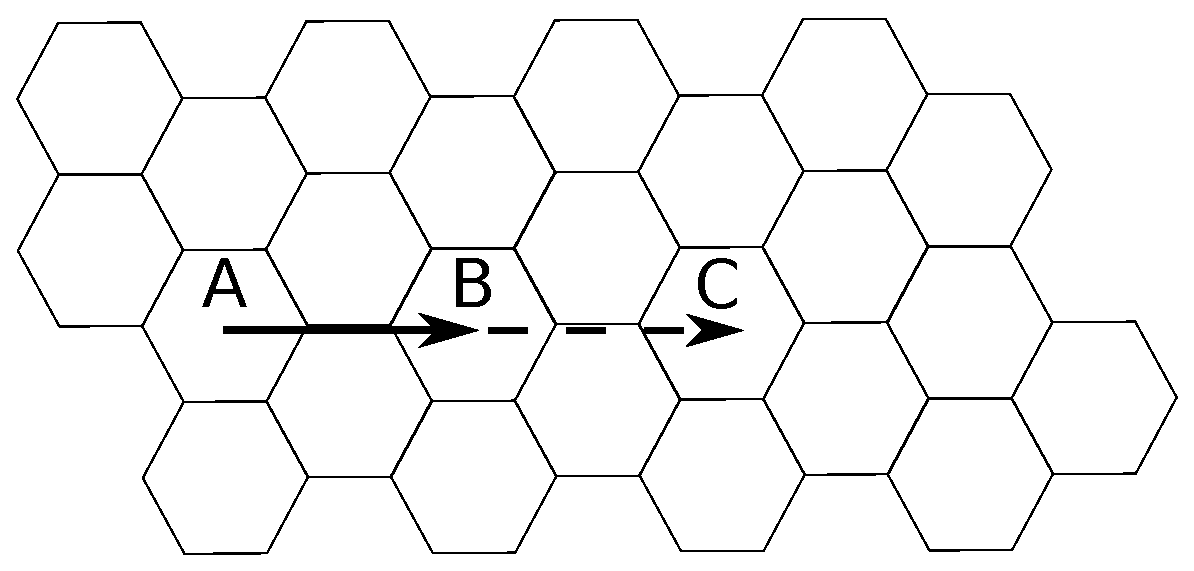
\includegraphics[width=0.5 \textwidth]{data/move_1.eps}  
  \caption{\footnotesize A ship moved from A to B in turn 1 will continue to C in
    the next turn if it does not accelerate due to gravity or burning
    fuel.}
\label{fig:1}
\end{figure}
\begin{figure}[h!]\centering  
  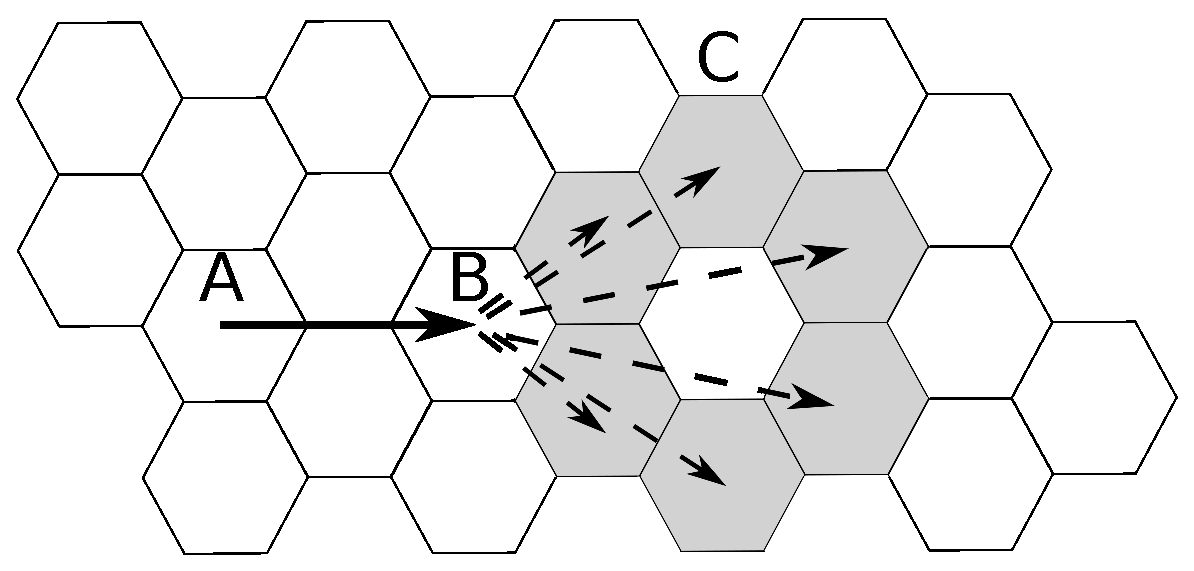
\includegraphics[width=0.5 \textwidth]{data/move_2.eps}  
  \caption{\footnotesize By burning one unit of fuel a ship may change
    the future tip of the vector by
    one hex.}
\label{fig:2}
\end{figure}
\begin{figure}[h!]\centering  
  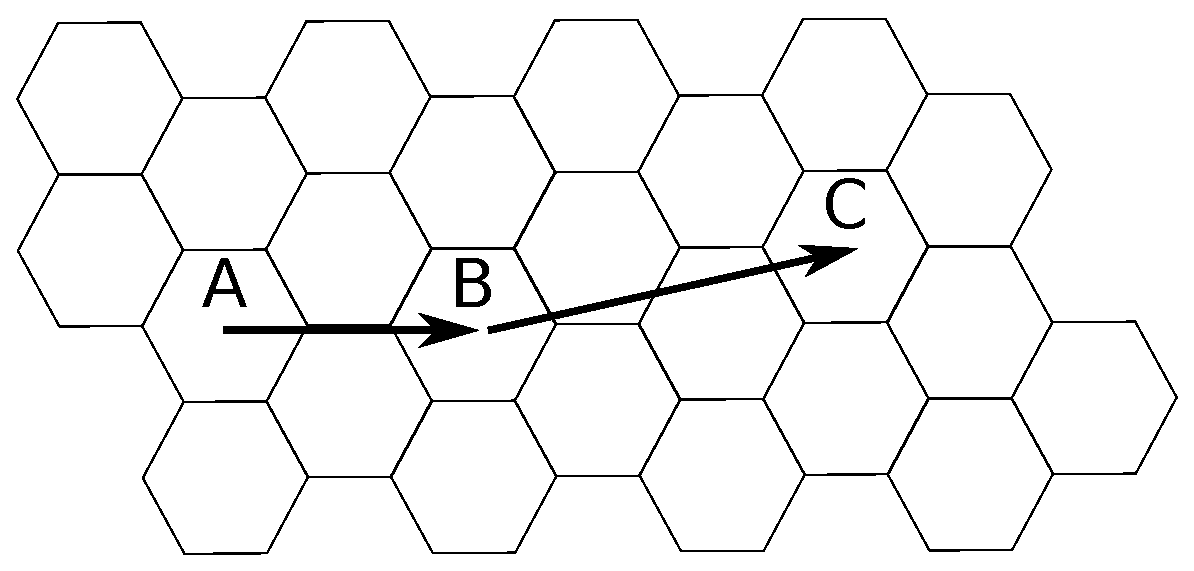
\includegraphics[width=0.5 \textwidth]{data/move_3.eps}  
  \caption{\footnotesize Here is the ship's final vector after having burnt fuel to
    change the vector to the ``north-eastern'' shaded hex in Figure \ref{fig:2}.}
\label{fig:3}
\end{figure}

\subsection{Gravity}

Stars and planetary bodies affect their surroundings through
gravity. Gravity is marked on the map as hexes with different types of 
arrows. On the turn \emph{after} a ship (or missile, mine etc) enters or passes through a gravity
hex, its vector is adjusted one hex in the direction of the arrow.  Several gravity hexes
can affect the vector each turn, the arrows are then just applied in
sequence. 

\begin{figure}[h!]\centering  
  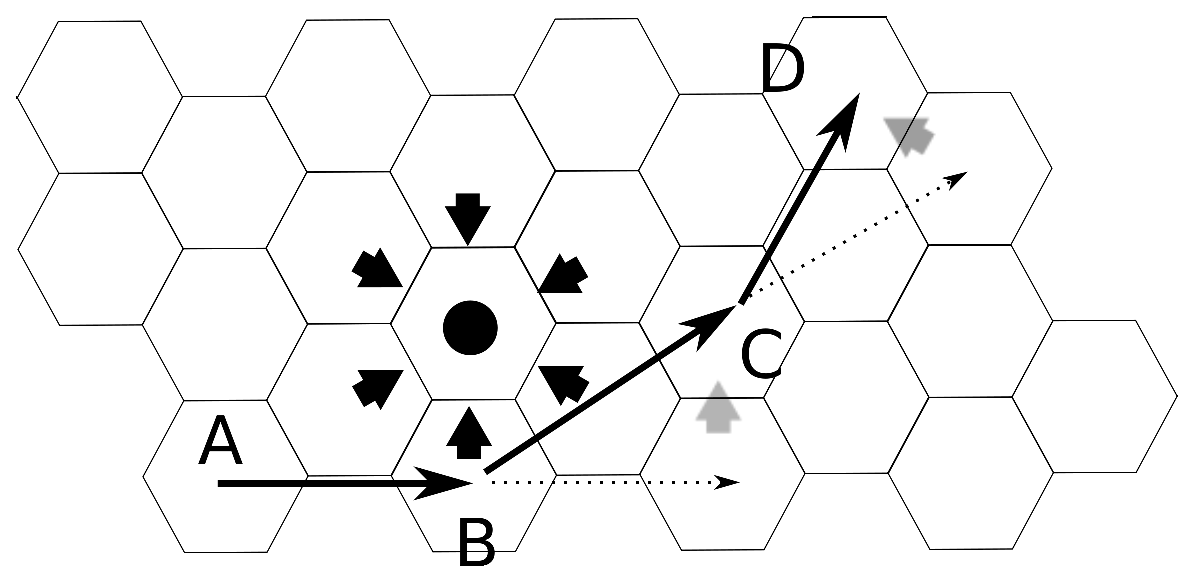
\includegraphics[width=0.5 \textwidth]{data/move_4.eps}  
  \caption{\footnotesize \emph{Effect of gravity}. Ship moves from A to B as normal, entering a
    gravity hex. 
    On the turn after (B to C), the vector's tip changes one hex
    in the direction of the gravity hex it passed on the turn
    before. Note that this new vector now also passes through a gravity
    hex. On the last turn, from C to D, the hex from previous turn adjusst
    the vector again. In this example the ship does not burn fuel, but
    if it did it would apply it after gravity corrections have been
    made each turn.}
\label{fig:4}
\end{figure}
\begin{figure}[h!]\centering  
  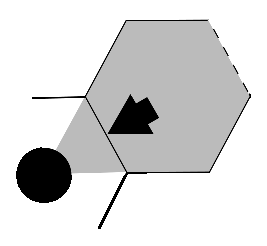
\includegraphics[width=0.10 \textwidth]{data/move_6.eps}  
  \caption{\footnotesize Ships passing between a gravity arrow and the gravitating
    object are affected by the gravity of the hex above. A
    ship passing exactly along the edge of a gravity hex is assumed to be
  affected by it \emph{except} if the edge is opposite to the arrow. 
  If a ship should happen to travel along a valid edge between two
  gravitational hexes, the arrow \emph{closest} to that edge is used.} 
\label{fig:6}
\end{figure}
% \begin{figure}[h!]\centering  
%   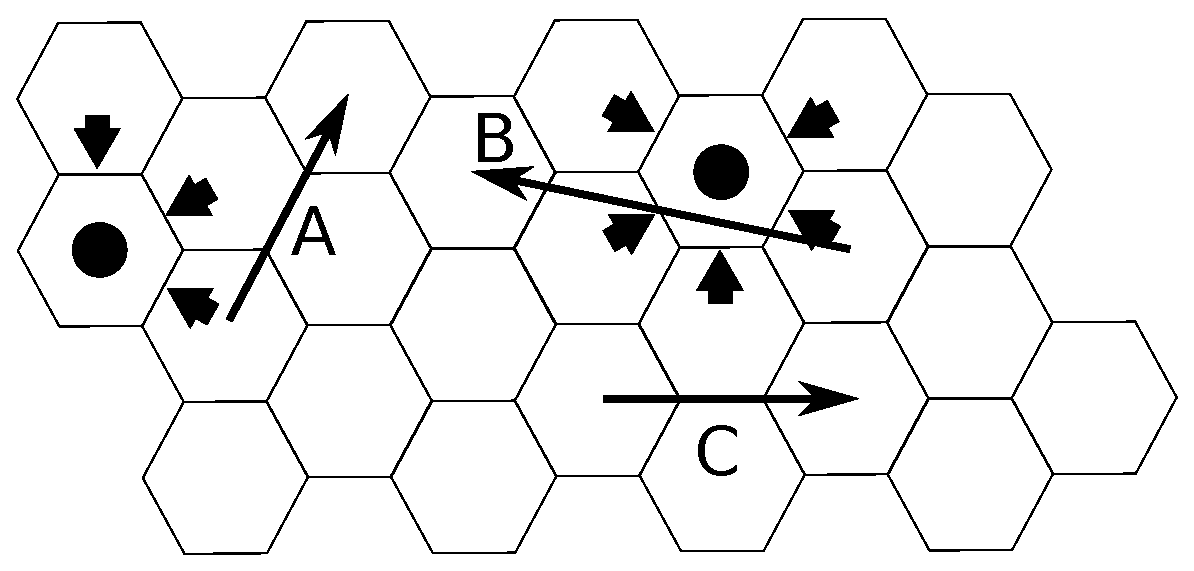
\includegraphics[width=0.5 \textwidth]{data/move_5.eps}  
%   \caption{Ship A is affected by two gravity arrows. Ship B is
%     affected by all three gravity hexes since the upward-pointing hex
%     also covers everything down to the planet surface. Ship C is not
%     affected by any gravity.}
% \label{fig:5}
% \end{figure}

\begin{figure}[h!]\centering  
  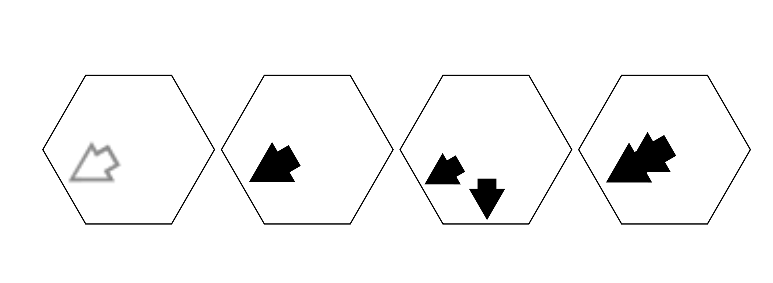
\includegraphics[width=0.5 \textwidth]{data/move_8.eps}  
  \caption{\footnotesize \emph{Gravity types}. From left to right: Weak gravity, normal gravity,
    two-directed gravity (choose which direction to apply) and double gravity.}
\label{fig:8}
\end{figure}

Apart from the normal solid black gravity hex described above, there
are three more types. 

\begin{itemize}
\item \emph{Weak gravity} is found around smaller moons and is marked with
  hollow arrows. If a ship enters a weak gravity hex, the player may
  \emph{choose} to apply that arrow or not. If not the hex is treated as
  empty space. However, if two weak gravity hexes are entered
  consecutively, the second hex's arrow entered \emph{must} be
  applied, regardless of what was chosen for the first arrow.

\item \emph{Two-directed gravity} is only found on the Sun. They are
  marked with two solid arrows in the same hex. They work like normal
  gravity, except the player must choose one (and one only) of the two
  arrows to apply.

\item  \emph{Double gravity}, marked by two overlying arrows, is found only
  around the Sun and shifts the tip of the vector two hexes in the
  direction of the arrow instead of just one.
\end{itemize}
\begin{figure}[h!]\centering  
  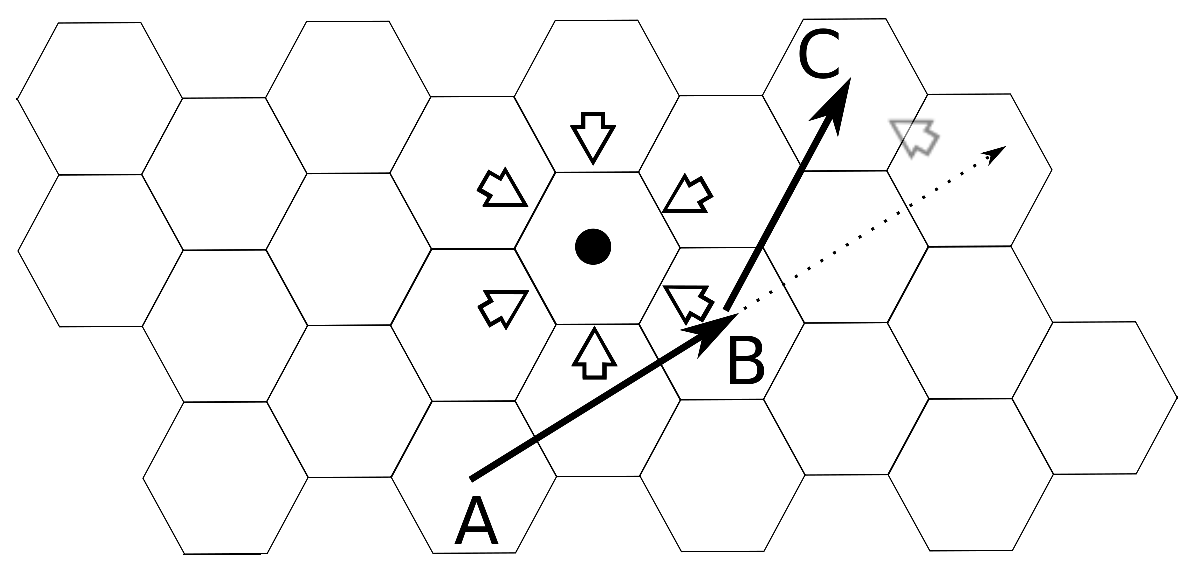
\includegraphics[width=0.5 \textwidth]{data/move_7.eps}  
  \caption{\footnotesize \emph{Weak gravity}. When passing through two weak gravity hexes, the second one
  to be entered always apply regardless of how the first one is
  treated (in this example the player chose to ignore the first hex,
  or point C would also have been shifted one hex upwards).}
\label{fig:7}
\end{figure}

\subsection{Entering Orbit}

TriAv allows for entering orbit around planets just using the normal
movement rules. This is done by entering orbit with a speed of
one, then burn fuel to break. You will then find you are orbiting
indefinitely without using any more fuel. The first turn the ship circles
without having to burn fuel is considered its first turn ``in orbit''.
When in orbit the ship may dock with orbiting bases to refuel and restock.

\begin{figure}[h!]\centering  
  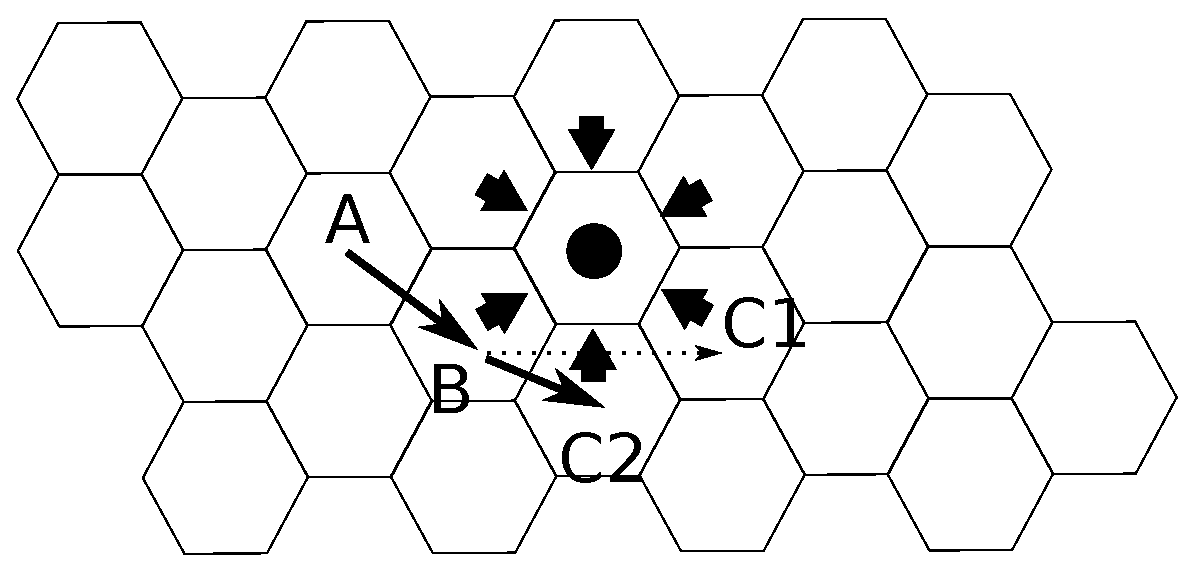
\includegraphics[width=0.5 \textwidth]{data/move_9.eps}  
  \caption{
\label{fig:9}\footnotesize \emph{Entering orbit.} Entering the vicinity of the
planet with speed 1 (A to B), the ship will on the next turn feel the effects of the
gravity arrow in hex B so as to try to accelerate it to point C1. If
the ship now burns fuel to break to C2 instad, it will find itsef in
orbit next turn, circling the planet without more use of fuel.} 
\end{figure}

\subsection{Planets}

A ship starting on a planet uses ground-supplied boosters to reach an
gravity hex above the planet's surface. This requires none of the ship's
own fuel. Once in orbit, the ship has zero speed and if it does not
spend fuel next turn it will crash back down onto the planet. 

A ship already in orbit may burn one fuel to land on the hex-side of the
planet it was above, assuming the game scenario allows it (like that
hex-side having a base or being friendly). When taking off again it
will do so from the same hex-side.  

If the vector of a ship intercepts the \emph{image} of a planet the ship is
assumed to have crashed and is destroyed. 

\subsection{Asteroids}

A ship may only safely pass an asteroid hex with a maximum
speed of one. If it passes at a greater speed, the player must roll
using the ``Asteroid'' collumn of the \emph{Other Attacks}
table. Asteroid bases are also considered to be asteroid hexes in
this regard, but ships accidentally cannot crash into an asteroid base
the way they can crash into planets.  


\subsection{Other ships}

Each hex in TriAv represents a very large volume of space, so any
number of ships can coexist in a hex without any problems. A ship whose
vector passes through the \emph{center} of a hex occupied by an enemy
ship may however choose to attempt to \emph{ram} the other ship. The
effect is rolled using the ``Ram'' collumn of the \emph{Other Attacks}
table. Damage rolled applies to \emph{both} ships equally. 

\subsection{Bases}

Bases are found on asteroids, on planet surfaces and in orbit around
planets. They may be military installations or points of commerse. 

When docked with or landed at a base, the player may buy fuel and
restock weapons assuming the scenario allows it. 

Orbital bases are marked with little dots above planet surfaces. A ship \emph{in
  orbit} that passes directly above an orbital base may
dock. Planetary bases are reached by landing on the correct hex side
(this requires burning fuel) whereas asteroid bases are visited by
simply coming to a stop in the asteroid base hex. Asteroid bases and
Planetary bases provide immunity against all enemy weapons \emph{except}
Space-to-ground weapons.  

\subsection{Leaving the map}

Leaving the map usually means the ship is eliminated from play. If
players agree beforehand one can instead allow for the ship to reappear at the
point of exit after an agreed number of penalty turns. It would return
with a speed of zero.  


\section{Combat}
\label{sec:combat}

With the weight-limitations inherent in any realistic spaceship design it is
impossible to add enough armour to match the cheap and terrible destruction
capabilities of space weaponry\footnote{If a tactical nuke detonates at point blank
range it doesn't really matter if you are a large battleship or a small frigate
-- the only difference is how large the scraps will be...}.

\subsection{Damage}
\label{sec:damage}

Whenever a launched weapon hits or guns are fired, the attacker rolls
a six-sided die, applying 
any modifications. The resulting number is matched to the correct
collumn of one of the two tables found on the printable
play-aid (\emph{Gun attacks} or \emph{Other attacks}).
Reading the result from the table, this may result in a miss or
various types of damage. 

The damage types, as found in the attack tables, are: 
\begin{itemize}
\item D\emph{n} - Disable ship \emph{n} turns. The ship continues on
  its current vector until it can restore normal operation. Gravity
  of course works as normal during this time. Ships
  cannot fire weapons when disabled\footnote{It is however sometimes assumed
    that large ships, like dreadnoughts, still can fire their guns even
    when disabled.}. This includes retaliation-fire against the
  attacker that disabled them.

  D-type damage do \emph{not} stack. The new D-type damage replaces the old
  one if it is larger than the number of disabled turns remaining from
  the old D-type damage. Otherwise it is ignored.
\item T\emph{n} - Targeted hit. Roll \emph{n} times to decide which
  ship subsystem was hit. For each of these hits, roll d6 again to see
  how much damage was applied to that subsystem. See Section
  \ref{sec:ship_manifest} for more information about the subsystems
  and about how damage is assigned to them. 
\item S\emph{n} - Structure hit. Roll a six-sided die \emph{n} times
  and apply the sum as damage to the \emph{Structure} subsystem directly.
\item E - Elimination (critical hit). The ship is immediately destroyed. 
\end{itemize}

\subsection{Launched weapons}
\label{sec:damage_launched_weapons}
These types of weapons are launched during the launch
phase, before the ship actually moves in the turn. 
They ``inherit'' the velcity vector of their launching
spaceship and their movements are plotted like a separate entity,
taking gravity into effect. It can be a good idea to plot launched
weapons with dotted lines to separate them from spaceships. When
hitting an ememy, damage is determined using the correct collumn from
the \emph{Other attacks} attack table.  

A ship may only fire one launched weapon per turn. 

Launched weapons lasts a maximum of five turns unless they hit something. 
At the beginning of the launching player's sixth turn they
automatically self-destruct. A launched weapon can also attack another
launched weapon. If the attack roll is anything but a blank result,
both weapons are destroyed. 
\\\\
\emph{Mines} are unguided clusters of explosives. Their nature
means that the launching ship \emph{must} make a burn maneuver to the
side in order to avoid running into the mines it just launched. 

Any spaceship being hit directly, or which during a subsequent turn
\emph{intersects any part of the Mine's current vector} is considered to
have hit the mine field. If the mine enters a hex with several ships,
\emph{all} ships (including friendly ones) must roll for possible
damage.     

\begin{figure}[h!]\centering 
  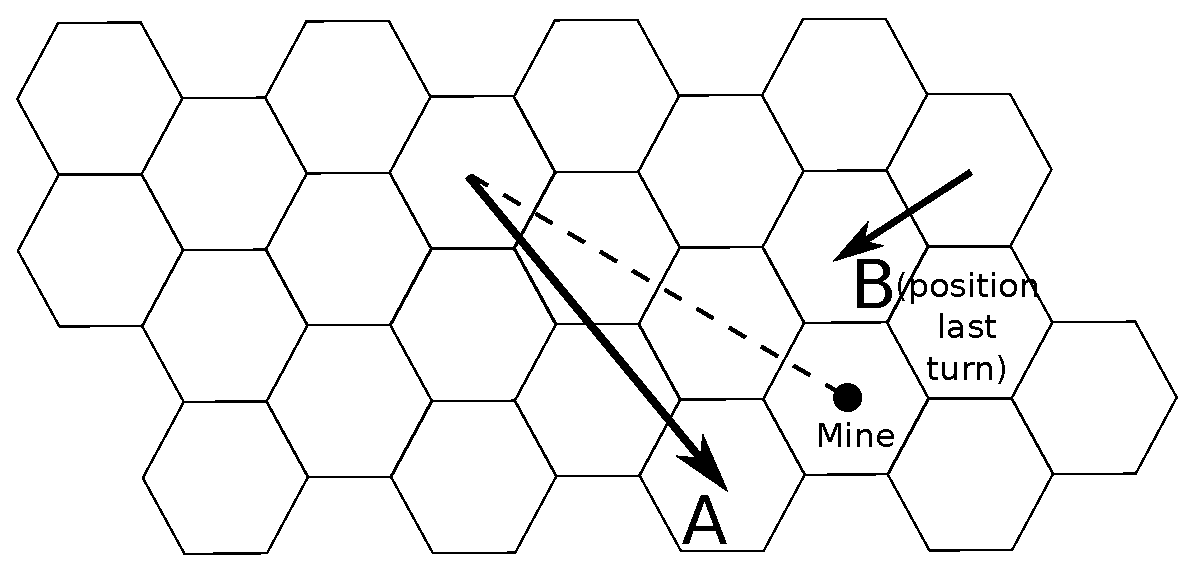
\includegraphics[width=0.5 \textwidth]{data/combat_1.eps}
  \caption{\footnotesize \emph{Use of mines}. In this turn,
    ship A drops a Mine (and boosts to the side to avoid 
    running into it itself). When it's B's turn, ship B will
    intersect the Mine's vector (and thus be hit) unless ship B
    changes its course. If it doesn't hit anything the mine will stay
    in space for another four turns.}
\label{fig:10}
\end{figure}

\emph{Missile weapons} are almost small spaceships of their own. The
payload generally being nuclear and big enough to seriously damage or outright
destroy any size ship, the main difference between missile types is
not so much the destructive capability as how good they are at 
hitting a target. 

To be hit by a missile, the enemy ship must either
be hit directly or on its move pass through the current \emph{head of the
missile's vector}. Missile weapons are intelligent
precision weapons and can separate friend from foe. The launching ship
can thus coexist with its own missile in the same hex without danger. If a missile
enters a hex occupied by several enemy ships, the attacking player may
choose which one it attacks (or even choose to just fly by!). 

\subsection{Guns}

Guns are massive mounted installations on the ship. They require large
amounts of energy and heavy 
mechanical foundations to launch their projectiles or beams of
energy. Guns use the \emph{Gun power} attribute. Gun power is a joint
description of how much of the ship's energy reserves and
infrastructure is devoted to the guns. The bigger a ship's Gun power
the more powerful can its guns be -- but the less mass is available
for equipping the ship.

Guns are fired on the Gun fire phase, after movement. The damage is
rolled with a d6 on the \emph{Gun attack} table and read in the
collumn matching the ship's Gun power.  

Each gun can only fire once per turn. If the ship has two guns, each
weapon may fire either on the same enemy or on separate
targets. This must be decided before any rolls are made and cannot be
changed regardless of the outcome of the first roll. The two guns are treated as
separate attacks (they do not stack).  

\begin{figure}[h!]\centering 
  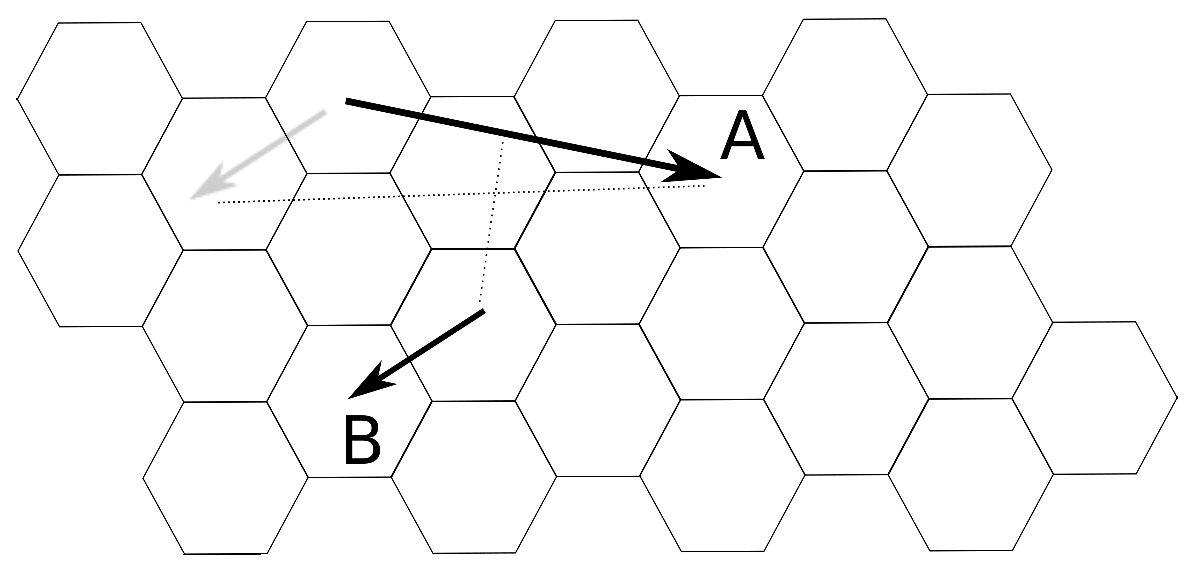
\includegraphics[width=0.5 \textwidth]{data/combat_2.eps}
  \caption{\footnotesize \emph{Calculating gun attack modifier}. Ship A fires
    on B. The distance
    between the ships are calculated at the closest point of their
    vectors to be 1 (which is less than 2 and thus ignored). The relative velocity is much bigger; by vector
    addition it is found to be 4, which is two bigger than 2. The
    attack roll is thus made with a -2 modification. } 
\label{fig:11}
\end{figure}

Guns are affected by the \emph{distance} to the target as well as its
\emph{relative velocity}. The distance is counted from 
the \emph{closest} point of contact between the two ships'
vectors. For every hex of distance \emph{greater than 2}, a -1 modififier
is applied to the attack roll. The relative velocity is found by
simple vector subtraction (shift one vector's base to the base of the
other and count the hexes between their arrowheads). Again, any
relative velocity greater than 2 adds a -1 modifier. 

Most ships with guns also have \emph{retaliation
  capability}. This means that once the attacking ship has attacked
and damage been applied, the attacked ship may fire back with its own
guns (assuming its guns allow it and the ship was not disabled or
destroyed in the first attack).   

\section{Ship manifest}
\label{sec:ship_manifest}

Each TriAv ship is created by filling out a \emph{Ship
  manifest} as seen in Figure \ref{fig:12}. 

\begin{figure}[h!]\centering 
  \fbox{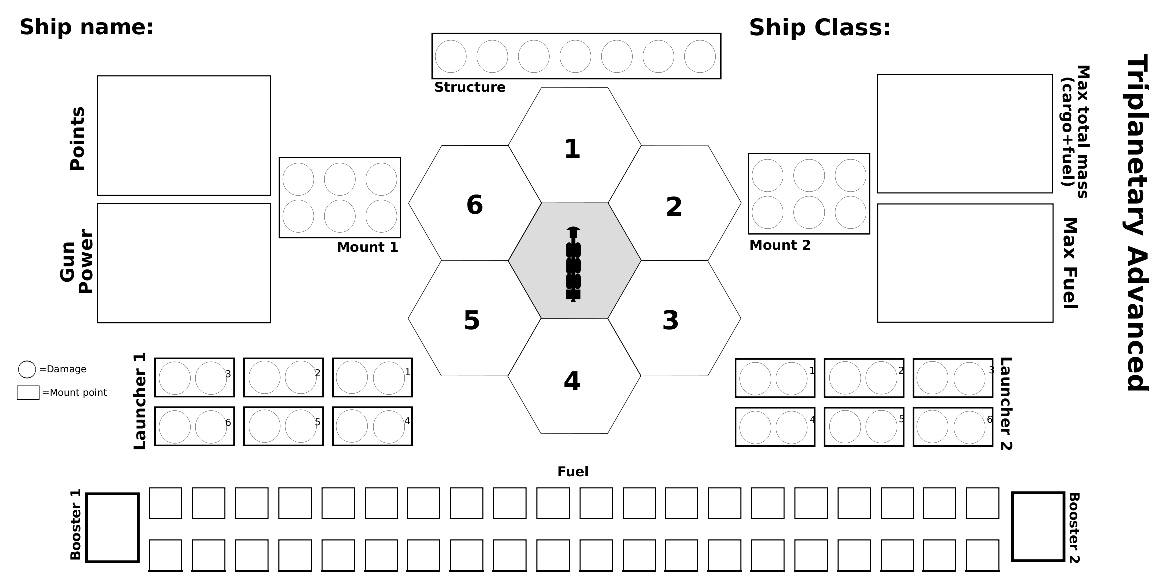
\includegraphics[width=0.4 \textwidth]{data/ship_1.eps}}
  \caption{\footnotesize \emph{The ship manifest}. } 
\label{fig:12}
\end{figure}

\subsection{Basic ship properties}

The ship manifest has four larger squares. These describe the basic
attributes used for creating and outfitting a ship. 
\begin{itemize}
\item \emph{Points} work like cash and are used for buying ship weaponry
  and equipment. Some game scenarios require players to also use points to
  buy the ship(s) they want to use. Often some points have to be saved in
  order to be able to afford refitting and refueling the ship during play. 
\item \emph{Gun Power} is a measure of the power of the ship's
  guns. The value is between 0 and 6 and changes the collumn you use
  in the \emph{Gun attack} table. A high gun power reduces how much
  overall mass the ship can carry.
\item \emph{Max fuel} is a measure of how much fuel a ship can carry 
  in its tanks. Each unit of fuel weighs one mass unit. This value is
  usually around 15-20 for a normal TriAv military ship.   
\item \emph{Max total mass} is a very important attribute. It
  describes how much mass the ship can carry \emph{including}
  the mass of its fuel. So if a ship has a Max total mass of 50 and
  has filled up 20 units of fuel, it can only carry an additional 30
  units of mass. 
\end{itemize}

\subsection{Ship subsystems}

The manifest has a central little image of a spaceship surrounded by
numbers in a hexagon shape. Each of the six locations around the
ship represents a certain ship subsystem. When equipping your ship you
decide which of the subsystems hold your weapons and equipment.  

When your ship get hit with the ``T'' damage type, as
described in Section \ref{sec:damage}, roll a die to determine which
subsystem was hit. Roll again to determine how much damage is applied
to that subsystem. 

\begin{figure}[h!]\centering 
  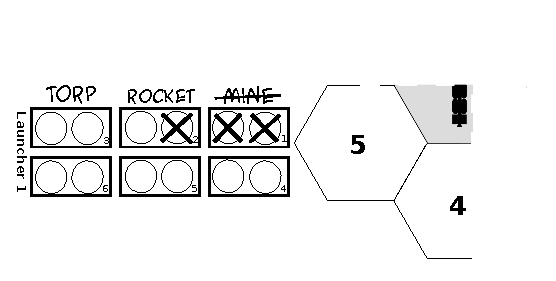
\includegraphics[width=0.5 \textwidth]{data/ship_2.eps}
  \caption{\footnotesize \emph{Subsystem damage}. After a 'T' type
    hit, the player rolled a '5' -- a hit on Launcher 1. The damage
    roll was '3'. Three circles were crossed out on the top row,
    beginning from closest to the ship. This destroyed the mounted Mine
    completely, but the Rocket is still operational.  } 
\label{fig:13}
\end{figure}

\begin{itemize}
\item \emph{Structure} (hit location 1) represents the frail central column of the
  ship, its command modules, computers and other vital systems. The
  Structure subsystem has 7 hit points (represented by circles); when
  all are gone the ship is destroyed. 
\item \emph{Mount 1 \& 2} (hit locations 6 and 2) can hold one Mounted weapon (like a gun
  battery) each. A mount has 6 hit points (represented by circles)
  after which the mount and weapon is destroyed. If there is nothing
  mounted there, the mount just represents armour. Excess damage given
  to the mount beyond the six hit points are applied to Structure. 
\item \emph{Launcher 1 \& 2} (hit locations 5 and 3) can each hold six launched weapons
  (represented by rectangles). The weapons loaded can be of mixed types and
  can be launched in any order. Each weapon slot has two hit points
  (represented by circles) making a total of 12 hit points per
  launcher. If a weapon looses its two hit points it is considered
  destroyed. Weapons are always mounted from the
  inside-out, top-to-bottom and damage is applied in the same way. If
  there is no weapon mounted where damage hits (or if the weapon was
  already launched), the damage is considered to
  have hit armour instead. If more than 12 damage is given to a
  Launcher, excess damage is instead applied to Structure. 
\item \emph{Fuel} (hit location 4) represents the fuel tanks of the
  ship. No ship can ever carry more fuel than its \emph{Max Fuel}
  attribute. As the ships accelerates, fuel is spent by ticking off
  the squares here. If damage is applied to the Fuel tanks, the result
  is always a loss of fuel -- as many units are lost as the damage
  given. If there are no more fuel units to loose, excess damage is
  applied to Structure instead. 
\item \emph{Booster 1 \& 2} These are not really considered subsystems
  since they cannot be damaged. Each booster slot can hold one
  single-use booster (so each ship can only carry a maximum of two
  boosters at any time).  
\end{itemize}

\subsection{Designing your own ship}

\emph{Gun power, Max fuel} and \emph{Max total mass} are properties of
each ship's design. To design a ship, first decide how much
fuel it should carry, and which Gun power it should have, then
calculate Max total mass with the following formula: 

\begin{eqnarray*}
  MaxMass = Engine \\ + (4\cdot MaxFuel) \\ - (10\cdot GunPower)
\end{eqnarray*}

\emph{Engine} is a value between 0 (default) and
40 and represents the use of a more efficient/more futuristic
engine. This will allow you to create a greater variety 
of ship designs\footnote{Consider Engine a fudge factor. You will
  find that very high Gun power will not allow you enough max mass to mount
  any guns unless you also put in a more powerful engine.}.
\\\\
\\\\
The \emph{Point} cost of a ship can be found from 
\begin{eqnarray*}
  Cost = Maxmass \\+ (10\cdot GunPower) \\+ (10\cdot EngineBonus)
\end{eqnarray*}
(But feel free to modify costs up and down after what is required for
the game). 
\\\\
If you don't want to design your own ships, Some
standard ship types and engine design examples are found on the
handout.  

\section{Equipment/Services}
\label{sec:equipment}

This constitues a brief technical description of the weapons and
equipments available to be bought from bases for mounting on a
ship. Each item has a point cost and a mass. How many points each
player has available is decided upon before starting play. The mass of
all equipment + fuel must never exceed the ship's \emph{Max total mass} attribute. 

\subsection{Repair}

This is not equipment but a service and has only cost, no mass. Buying
a unit of repair will dispatch the base's technicians and robots to
work on patching the ship up, restoring one point of damage from any subsystem\footnote{The
  only exception is lost fuel, which is simply recovered 
by buying more fuel...}. However, repairing a spaceship is complicated
work -- every unit of repair bought will effectively \emph{disable}
the ship for one subsequent turn as repair crews work on it. 

A ship buying the repair from an orbiting base will continue to orbit
as normal while being repaired, for as many turns as needed.

A player may choose to abort the repair cycle prematurely (and get their
money back) if the situation so requires. 

\subsection{Fuel}

Fuel is the life blood of any spaceship. Each unit of fuel has mass of
1 and each ship cannot carry more fuel than is allowed by its
\emph{Max Fuel} property. A ship can only burn one unit of fuel per
turn to change its velocity. A ship can opt to carry less fuel than
their maximum, e.g. in order to fit additional weaponry. 

\subsection{Boosters}

Boosters are single-use systems that gives the ship a temporary extra
acceleration. Using a booster does not expend any fuel (it carries its
own fuel), but in addition to using the booster the ship can also burn fuel
as normal if desired. Each ship can carry a maximum of two boosters (in the
Booster 1 \& 2 slots). 

\begin{itemize}
\item \emph{Chemical booster}. This is a pack of rockets with solid
  propellant, pretty much like huge firework-rockets that are ejected
  once they burn out. Chemical boosters supply 1 additional point of
  thrust when used. 
\item \emph{Orion booster}. This powerful single-use system integrates a
  deployable absorber plate with a nuclear charge of several kilotons. The
  nuclear weapon is ejected just behind the spaceship and
  detonated. The absorber plate protects the ship while converting the
  energy of the blast into a powerful acceleration\footnote{This may
    sound  bizarre, but a variant of this has been seriously
    considered for a full ship drive.}. An Orion booster supply 2
  additional points of thrust in the turn it is fired.  
\end{itemize}

\subsection{Launched Weapons}

Launched weapons are mounted in the Launcher 1 or 2 subsystems on the
spaceship. All launched weapons self-destructs after 5 turns. All
launched weapons except Mines and EMP attack with the ``Missiles (any)''
collumn of the \emph{Other damage} table. Launched weapons may attack
other launched weapons - any hit (including disabling hits) will
destroy both weapons. 

\begin{itemize}
\item The \emph{Mine screen} is a small automated probe dispersing a vast
  screen of deadly unguided explosive charges around it, intended to
  maximize hit probability. Mines are unguided, so the launching ship
  must also avoid them. Mines are not as destructive as other launched
  weapons, but they are easier to hit with (See Section
  \ref{sec:damage_launched_weapons}).  They make for powerful
  strategic weapons to restrict the movements of an enemy. 
\item \emph{Rockets} are relatively simple deep space weapons carrying
  a standard nuclear warhead. It has its own rocket engine and
  sensors, but having only a small fuel supply, rockets may only apply
  up to 1 point thrust at the moment of launching from the ship, after which it
  will cruise until it hits something or self-destructs. 
\item \emph{EMP rockets} essentially consists of the same chassis as
  rockets but has its warhead replaced with a nuclear charge tuned
  to release energies causing maximum harm to electrical
  components. EMP rockets will not cause any direct damage to an enemy
  but can disable them for a longer time 
  than any other weapon type, making it a powerful support weapon.  
\item \emph{Missiles} are bigger than rockets but work along the same
  principles. Their bigger engine and fuel supply allow them up to 2
  points of thrust at the moment they are launched from the ship. 
\item \emph{Torpedos} are intelligent stealth weapons capable of being
  dropped out of their launch tubes to drift through space until the
  right time has come to fire its engine. A torpedo has one point of fuel to spend,
  just like a rocket, but may apply that thrust at \emph{any time} during its
  flight. 
\item A \emph{Booster Torpedo} is a torpedo with extra fuel tanks. It
  has two units of fuel which it can use at any time during its
  flight. 
\item The \emph{Fusion bomb} is a tactical weapon. It is a
  massive, sleek bullet that can strike base armour or 
  enter planetary atmospheres to take out hardened bunkers. It has no thrust
  capabilities on its own and cannot be used against ships (or other
  launched weapons, although it can be attacked by the latter). The
  only target it can be used against is planetary installations or
  orbital stations.  

  A fusion bomb hitting a planet hex side will destroy any base
  located there. The attacking player can choose to destroy an orbital
  base instead of hitting the planet's hex below. A hit on an asteroid
  base will destroy that base, converting its hex into a normal
  asteroid hex. All ships docked (or at rest) at attacked bases will
  be destroyed along with the base, but not ships that happens to be
  passing by in the same hex.

\end{itemize}

\subsection{Mounted weapons}

These weapons can be mounted in the Mount 1 or 2 subsystems of the
ship. A ship can have a maximum of two mounted weapon systems at any
time. Both guns can then fire independently at two targets or twice at
the same target. 

\begin{itemize}

\item \emph{Railguns} use a catapult-like rail system to electromagnetically launch a
  metallic slug at terrifying speeds. The projectile is just a dumb chunk of metal --
  the kinetic energy released upon a direct hit is enough to punch
  through anything. Ammunition is virtually infinite. But even though
  the slugs travel fast, even a minute course change by the enemy while the slug
  travels will cause it to miss by hundreds of kilometers. 
\item \emph{Heavy Rail cannons} does not fire
  heavier projectiles than railguns, rather it has a much heavier
  support structure that allows them to fire the slug with higher speed. A
  shorter time for travelling down the rail means higher precision. A
  heavy railgun gives +1 to the attack roll. The heavier mount however
  makes the ship loose its ability to retaliate when fired upon.
\item \emph{Laser batteries} use large capacitors to discharge a
  powerful pencil-thin beam of X-ray radiation across
  space. Delivering this energy to a point on the target quickly cooks
  through any defenses. The stubby laser turret itself is not very
  heavy, the problem is the massive energy requirements for each
  shot. A laser battery \emph{ignores} any effects of relative
  velocity on its attack roll.
\item A \emph{Mass driver} is a electromagnetic railgun stretching the
  full length of the ship, designed to launch a heavier sliver of
  metal. Sometimes considered as a type of spaceship drive in itself,
  the kinetic energy delivered by a massdriver slug is tremendeous. A
  massdriver gives a +2 to the damage roll. Its structure however
  makes it unsuitable for retaliation-fire. 
\item \emph{Flak decoy guns} are defensive weaponry. These automatic
  guns fire shrapnel ammunition that fill the space around the
  aircraft with small objects, expanding gas and pencils of laser light in order to
  confuse or even destroy the sensors or control systems of incoming missiles. Every Flak
  decoy gun reduces the attack roll of any missile (but not mines) by 1). 
\item \emph{Emergency thrusters} are extra chemical rockets mounted
  around the cicumference of the ship. When fired upon by ballistic
  weapons (or lit up by a laser point) the emergency thrusters fire
  randomly to make the ship's exact position harder to track. Each
  pack of emergency thrusters reduce Gun attack rolls by 1. 
\end{itemize}


\section{Optional rules}
\label{sec:optional_rules}


\subsubsection*{Fewer sitting ducks}

Whereas it may be realistic that a disabled ship is a sitting duck
against further attack, situations may arise where an attacking ship
keeps an enemy disabled indefinitely without any chance of
defence. This can be boring and frustrating for the player. The
following optional rule sections, used both or separately, may help
alleviate this:  
\\\\
An already disabled can \emph{not} be disabled again. If another
D-type damage is applied to a disabled ship, it is ignored. Other
types of damage are applied as usual. 
\\\\
After half the disabled time (rounded down) a ship's weapons come back
online and work normally.


\subsubsection*{Space rendevouz}

By matching vectors (speed and position), a ship may attempt to get
into physical contact with another ship.  Both ships must willingly
accept the space rendevouz for it to happen. Fuel and launched
weaponry (but not mounted weapons) may be exchanged between the two
ships, assuming they can carry the mass. If more than 20 units of mass
in total are moved between the ships, both ships must skip a turn to
complete the move. Also Points (i.e. money) can be exchanged between ships if the
players agree (Points have no mass). 

This rule allows for refuelling tankers and other supply ships as well
as allies helping each other out. 

\subsubsection*{Surrender}

This allows for a Space rendevouz, as above, between enemy ships,
where one of the ships have surrendered to the other ship. The
conditions of the truce is agreed on beforehand by the players --
usually how much loot the winner is allowed to take from the defeated
ship, or how many Points should be transferred. A surrender is
considered a binding bargain for both sides. The surrendering ship may not fire
upon the approaching ship and whatever prize was promised will be
transferred as agreed. Same rules apply to tranferring mass between
ships as for the Space rendevous rule. 

\subsubsection*{Boarding}

By matching vectors (speed and position) with a \emph{disabled} enemy ship, a ship may
attempt to launch a boarding party to subjugate it. Both players roll
a die; if the attacking player roll the highest, the enemy is
defeated, otherwise the defender has fought off the attack. Only one
boarding attempt can be made every turn, and \emph{only} if the
attacking ship is not performing any other attacks. It may also not
counterattack. 

If the enemy is defeated, the scenario may decide what happens; it
could be anything from being allowed to loot the enemy ship (same mass
limitations apply as for the Space rendevouz rule above) to the
attacking player now playing the enemy ship as their own. 

\subsubsection*{Civilian ships}

By defining some ships to be ``civilian'' one can define all sorts of
interesting scenarios. Civilian ships can carry weapons in their cargo
holds but cannot launch them. They can represent supply
ships or targets to raid if used with the Space rendevouz or Boarding
rules respectively. 

\subsubsection*{Special Asteroids}

The coloured asteroids around Clandestine are impassable unless you
know the exact route. Only ships belonging to the side that controls
Clandestine may enter these hexes, others are considered to have
crashed. Missiles entering a special asteroid hex detonates harmlessly
without affecting ships in that hex (ships \emph{already inside} such a hex can
however fire out. Cannons work both ways). A Fusion bomb will destroy a hex
of special asteroids (again without affecting ships), converting the
hex into empty space. 

\subsubsection*{Bases pick sides}

Bases can be assigned to a ``side'' and count some of the players as
enemies. All bases have a \emph{zone of control} with is marked with a
coloured outline on the map. Ships on the edge of such a zone is
considered to be inside the zone. It is impossible to dock and
refuel/restock at an enemy base unless this is especially defined in
the current game scenario. Bases act first of all on the
board\footnote{Meaning that ships tend to react to the actions of bases and
  not the other way around.}. 

Bases may have defences. A base can fire
a launched weapon of type \emph{Missile}(see Section
\ref{sec:equipment}) every two turns, or as often as defined in the
scenario. The base is assumed to have an infinite amount of missiles. 
All weapons are affected normally by gravity. 

Bases are generally equipped with one (or more) \emph{Mass driver}
(Again, see Section \ref{sec:equipment})
type guns. Bases may not fire its guns at ships outside its control
zone range.  

The only weapon capable of harming a base is a Fusion bomb. 

\subsubsection*{Mine fields}

Mine fields may be deployed depending on the scenario. They consists
of stationary \emph{Mine} weapons located in space at the
beginning of play. They most often have zero speed. A mine in a mine
field use the same attack table as a launched Mine, but is not
destroyed after 5 turns, it will last until it hits something. 

\subsubsection*{Fog of war}

This is mostly suitable for campaign scenarios and simulate a lack of
knowledge about the enemy loadout. Players don't reveal their ship manifests to each
other. Launched weapons are announced and drawn openly when fired;
also attacks with guns will reveal the ship's Gun power attribute. 

Each ship has a detector range or 3 hexes, only when coming closer
than this from each other do the two detecting players show each other
their manifests.  In the case of bases belonging to a
particular side, a ship passing within their detector range will also
reveal the ship's manifest to all players on the base's side. 

Fog of war is mostly suitable for bigger scenarios. One can envision a
fleet masking their movements by deploying unarmed empty ships as
decoys. 


\section{Game scenarios}
\label{sec:game_scenarios}

These are some simple game scenarios for quickly getting going. There
is not much ``story'' to these; they are simply
fun setups for a quick game. One can easily invent more elaborate
scenarios and campaigns. 

\subsection{Training}

For getting to learn the movement and gravity rules, newbie players
may get going with the following initial scenario.

\subsubsection*{Setup}
Everyone starts with a Corvette-class ship (Max total mass 70, Max
fuel 20, Gun power 1) and 20 fuel points (full
tanks). No other equipment and no weapons. They start on Earth and are
assumed to launch with boosters into an orbital hex of their choice on
the first turn.   

\subsubsection*{Goal}

Goal is to enter at least one gravity hex around
Venus, Mercury and the Moon -- in that order. The winner is the first
one to return to proper orbit around Earth. 

\subsubsection*{Special rules}
Ramming is not allowed. Refuelling at any orbital base is free. 


\subsubsection*{Variations}

For full training in more aspects of the game, add a railgun, a mine and a
rocket to all player's ships and let those also be restocked for free
at bases. Let the control zones around the planets be no-fire
zones. 

\subsection{The great planet race}

\subsubsection*{Setup}

All players start with one Frigate class ship (Max total mass 70, Max
fuel 20, Gun power 2, Engine 10). They have 200 points for outfitting
their ships as they see fit. Players start on Earth and launch with
boosters into an orbital hex of their choice on the first turn. 

\subsubsection*{Goal}

The goal is to touch the gravity wells of all major bodies
(i.e. bodies with normal gravity arrows, including the Sun) in the
solar system. The first to return to Earth and get into a stable orbit
wins. 

\subsubsection*{Special rules}

The control zone around Earth (green line) is a no-fire zone at the
beginning of play. Noone may launch weapons or guns from it or into
it.  Whenever all players have left the zone it ceases to exist for the rest of the
game. 

\subsubsection*{Variations}

Defining a particular order planets must be visited will create choke points and
will be much deadlier since ships get closer to each other. 

For a much calmer game, let all planets' detection zones be no-fire
zones throughout the game, only allowing weapons fire in deep space. 

\subsection{Last man standing}

\subsubsection*{Setup}

All players start with 300 points and may buy any ship and loadout
they can afford. All players start in space with speed 0. Ships's
starting positions should be in a large circle with roughly the same distance between
each ship. Size of the circle depends on how many players are
involved. 

\subsubsection*{Goal}

The winner is the last one alive. 

\subsubsection*{Special rules}

All bases are friendly and usable by everyone. 

\subsubsection*{Variations}

Instead of last man standing, one can also let destroyed ships ``pop''
back onto the map at their initial position d6 turns after they were
destroyed. Winner is instead the first one to score a pre-determined number of
kills. With many players this variation helps to avoid players sitting idle 
because they were eliminated early on. 

\subsection{Industrial sabotage}

Mercenaries are hired by a competitor to steal the valuable data from a
science vessel before the company can make use of it.

\subsubsection*{Setup}

The players are divided into two groups, the Guards and the
Mercenaries. If uneven, there should be more Mercenaries than
defenders. The Mercenaries fly Corvette class ships (Max total
mass 70, Max fuel 20, Gun power 1). Guards fly Frigate class ships (max total mass 70, Max
fuel 20, Gun power 2, Engine 10). Mercenaries have 100 Points for
buying equipment, Guards have 150. 

The Guards protects an unarmed science ship. This civilian ship has
Max fuel 20 and cannot carry any extra cargo. 

All defenders and the civilian ship start \emph{in orbit} around Earth,
at any hex and orbiting direction desired. Same goes for the
Mercenaries, except they orbit Mercury.

\subsubsection*{Goal}

The science ship must touch the gravity wells of Venus and Mars (in
any order) before docking with the orbital research base on Io
(must be the last stop).  If it suceeds without the ship being
boarded, Guards win a clear victory. 

Mercenaries win a clear victory if they manage to board the transport
and subjugate its crew, to then manage to escape with the stolen information
back to touch the gravity well of Mercury. 

If the transport is destroyed before it completes its journey (and
without its secrets having been stolen) the game is considered a weak
win for the Mercenaries. 

If the secrets are stolen, but the Mercenary ship is destroyed before
reaching Mercury, the game is assumed a draw unless the science ship
does manage to complete its trip, in which case it's a weak victory
for the Guards.  

\subsubsection*{Special rules}

The civilian ship moves last of all ships. Its movements are normally jointly
agreed upon by the defender players. But every \emph{5th} turn it is instead
controlled by the Mercenaries! Mercenaries may not use a boost
that causes the ship to be immediately destroyed. 
\\\\
The Boarding rules are used. If the boarding suceeds, the boarding
Mercenaries ship is assumed to carry the important data with it. The
ship can be boarded any number of times to re-obtain the information. 
\\\\
If the civilian ship should exit the map, it is assumed to ``bounce''
off the edge, returning back into the map again with the same speed as
before but with its direction mirrored. Other ships behave like normal.

\subsubsection*{Variations}

The scenario may be too difficult for the Mercenaries (especially the
docking part). By making the Mercenary control the civilian ship more
often (say, every fourth or even third turn) one can make its
behaviour more erratic and difficult to protect by the guards. 


\subsection{Hostile takeover}

Two mega coorporations have moved from sabotage and espionage to full
scale war.  

\subsubsection*{Setup}

The players are divided into two groups. One group controls the
orbital base of Io, the other side controls one of the two bases of
Mercury (the one facing Earth). Mars' bases are assumed neutral and
available to all. All other bases in the solar system are closed to
the warring factions while the conflict is going on. Equipment is
bought normally at all available bases. 

Each player gets 400 points to buy ship(s), using any loadout except
Fusion bombs. 

Each faction's home base starts with one free-of-cost Fusion bomb in stock. 

Upon start of play, each home base may deploy one Mine up to two hexes
away, with a speed of zero. This mine follows the \emph{Mine fields}
optional rule and is not destroyed after 5 turns. 

\subsubsection*{Goal}

The goal is to hit the enemy's headquarter with a Fusion bomb. 
If both bases are destroyed within two turns of each other the result
is considered a draw, otherwise it is a decisive victory for the side
first destroying their target.

\subsubsection*{Special rules}

Optional rules \emph{Fog of war}, \emph{Mine fields}  and \emph{Bases
  pick sides} are used. Bases may launch \emph{Missiles} every five
full rounds  (one round being when all players have moved once) and
each also has a \emph{Mass driver} gun.  

Each base produces a \emph{Fusion bomb} every 10 full rounds. A ship must be docked to the
station to load a Fusion bomb. A bomb loaded from the home base is
free of charge.

\subsubsection*{Variations}

Closing Mars and opening some of the other bases for neutral use
changes the tactical situation somewhat. For complete mayhem, let
bases fire missiles more often. 




% ============================================================================================= Document End
\end{document}






